

\section{Problema 2}
\subsection{Inciso \textit{d}}

\begin{figure}[H]
	\centering
	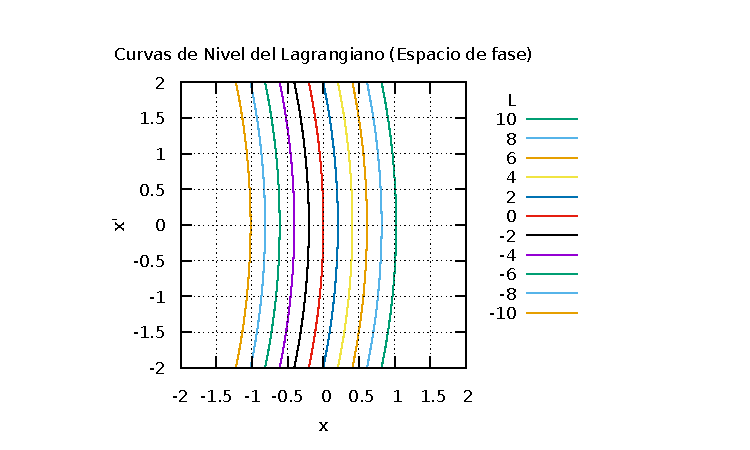
\includegraphics[scale=1.05]{problema2d.pdf}
	\label{2d}
	\caption{Curva de Nivel del Lagrangiano}
\end{figure}



\subsection{Inciso \textit{e}}

\begin{figure}[H]
	\centering
	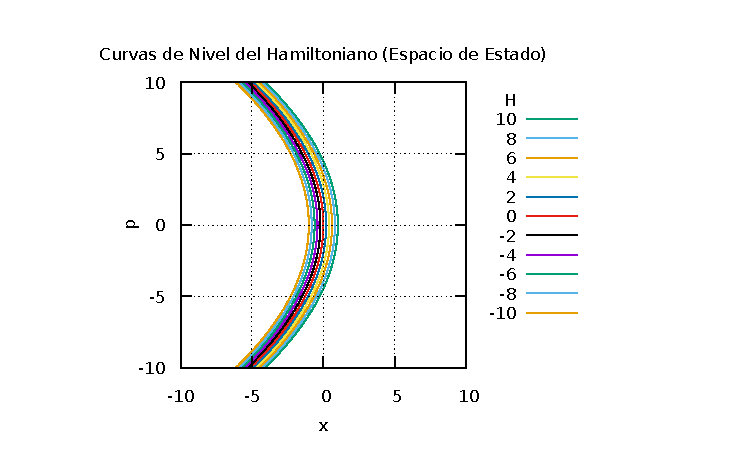
\includegraphics[scale=1.05]{problema2e.pdf}
	\label{2d}
	\caption{Curva de Nivel del Hamiltoniano}
\end{figure}









\section{Problema 3}
\subsection{Inciso \textit{d}}

\begin{figure}[H]
	\centering
	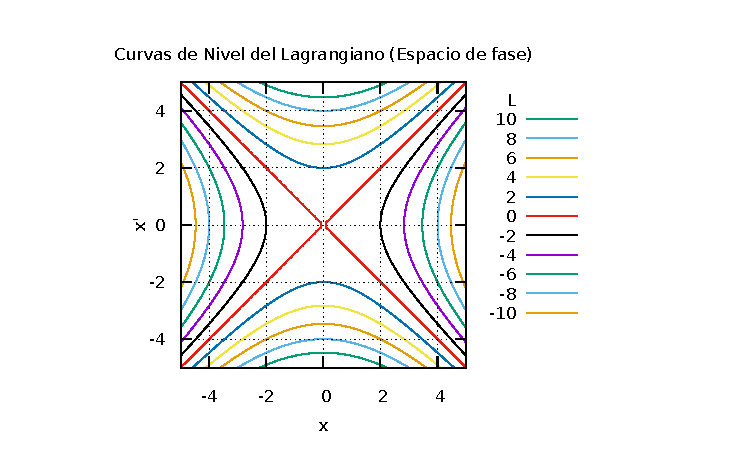
\includegraphics[scale=1.05]{problema3d.pdf}
	\label{2d}
	\caption{Curva de Nivel del Lagrangiano}
\end{figure}



\subsection{Inciso \textit{e}}

\begin{figure}[H]
	\centering
	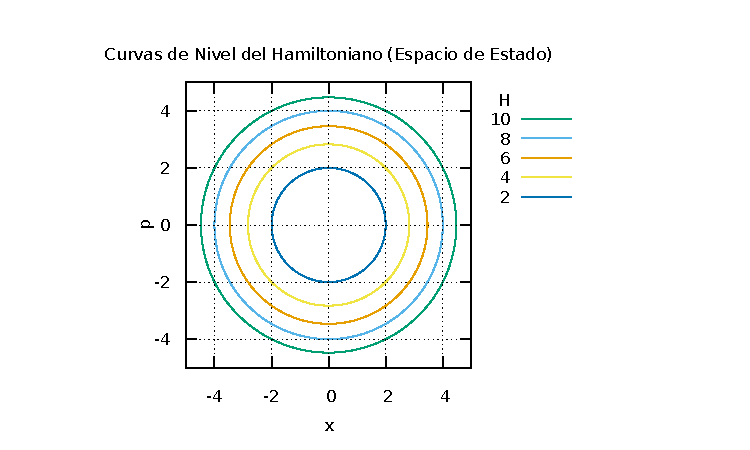
\includegraphics[scale=1.05]{problema3e.pdf}
	\label{2d}
	\caption{Curva de Nivel del Hamiltoniano}
\end{figure}







